A covariance function, or kernel function is a key part of the model used. Since not any function linking two inputs $x$ and $x'$ will in general be a viable kernel function, necessary, as well as useful properties of kernel functions need to be discussed. First, kernel functions must be positive semidefinite, 
\begin{equation}%positive semidefiniteness of kernel functions
	\int k(\bm{x},\bm{x'})f(\bm{x})f(\bm{x'})d\mu(\bm{x})d\mu(\bm{x'}) \geq 0.
\label{eq:positive_semidefiniteness_of_kernel_functions}
\end{equation}
Here, $\mu$ denotes a respective measure. Kernel functions also can be stationary, when it is a function of $\bm{x} - \bm{x'}$, exhibiting translation invariance in input space. A kernel function can be isotropic, a function of $|\bm{x} - \bm{x'}|$, making it invariant to all rigid motions. Isotropic kernel functions are also known as radial basis functions (RBF). If the kernel function is a function of $\bm{x} \cdot \bm{x'}$, it is called a dot-product kernel function. These are invariant to a rotation of coordinates about the origin, but not translation. Kernel functions also are the underlying reason for some properties concerning the total process, e.g. mean-square continuity and differentiability. \newline
\textbf{Continuity:} Continuity is a property of the Gaussian process, directly exhibited from the choice of kernel function. A stochastic process is continuous, if in a sequence of points $x_1, x_2, ..$ with another fixed point $_x*$ in $\mathbb{R}^D$ $|\bm{x}_k - \bm{x}_*| \to 0$ as $k \to \infty$. Then a process $f(x)$ is continuous in mean-square at $x_*$ if $\mathbb{E}[|f(x_k)-f(x_*)|^2] \to 0$, as $k \to \infty$. If this holds for all $x_* \in A$ where $A$ is a subset of $\mathbb{R}^D$, then $f(x)$ is said to be continuous in mean square over $A$. A random field is continuous in mean square if and only if its covariance function is continuous at $x=x_*=x'$. 
For stationary covariance funtions this reduces to checking continuity at $k(0)$. \newline
\textbf{Differentiability:} Using the mean square derivative of $f(x)$ in \textit{i}th direction 
\begin{equation}%mean square derivative of i-th direction
	\frac{\partial f(x)}{\partial x_i} = \lim_{h \to 0} \frac{f(x+h\bm{e}_i)-f(x)}{h},
\label{eq:mean_square_derivative_of_i-th_direction}
\end{equation}
and checking if the limit exists for order $2k$ and is finite at $x=0$, then the \textit{k}th order limit exists as a mean square limit. Here, the properties of the kernel around $0$ determine the smoothness properties of a stationary process. \newline \newline
Following, some of the more prominent kernel functions are presented, with some practical properties. Almost all of the following are stationary and non-degenerate, meaning they are stationary and of infinite rank.\newline
\begin{equation}%linear kernel function
	k_{linear}(\bm{x_i}, \bm{x_j}) = \sigma^2 \bm{x_i}^{\top} \cdot \bm{x_j} 
\label{eq:linear_kernel_function}
\end{equation}
is the linear kernel. As the most simple of kernels, it is as an exceptional case in this listing neither stationary, nor non-degenerate. 
\begin{equation}%exponential kernel function
	k_{exp}(\bm{x_i}, \bm{x_j}) = exp(-\frac{1}{2l}d_{ij}),
\label{eq:exponential_kernel_function}
\end{equation}
the exponential kernel, where $d_{ij} = ||\bm{x}_i - \bm{x}_j||_2$ is the Euclidian distance between the input arguments. 
\begin{equation}%squared exponential kernel
	k_{sqe}(\bm{x_i}, \bm{x_j}) = exp(-\frac{1}{2l^2}d_{ij}^2)
\label{eq:squared_exponential_kernel}
\end{equation}
is the squared exponential kernel. It is also known as radial basis function. 
\begin{equation}%matern 32 kernel
	k_{mat32}(\bm{x_i}, \bm{x_j}) = \Bigg( 1 + \frac{\sqrt{3}d_{ij}}{l} \Bigg) exp \Bigg( - \frac{\sqrt{3}}{2l} d_{ij} \Bigg)
\label{eq:matern_32_kernel}
\end{equation}
is the Matern3/2 kernel. it is a special case like the Matern5/2 kernel
\begin{equation}%matern 52 kernel
	k_{mat52} = \Bigg( 1+ \frac{\sqrt{5}d_{ij}}{l} + \frac{5r^2}{3l^2} \Bigg)exp\Bigg( \frac{\sqrt{5}d_{ij}}{l} \Bigg)
\label{eq:matern_52_kernel}
\end{equation}
of the Matern class of kernels
\begin{equation}%matern kernel class
	k_{mat} = \frac{2^{1-\nu}}{\Gamma(\nu)} \Big( \frac{\sqrt{2\nu}d_{ij}}{l} \Big)^\nu K_\nu \Big( \frac{\sqrt{2 \nu}d_{ij}}{l} \Big) .
\label{eq:matern_kernel_class}
\end{equation}
The matern kernels can be constructed with positive parameter $\nu$, $K_\nu$ is a modified Bessel function. Also, as $\nu \to \infty$ the function becomes the smooth squared exponential kernel, for $\nu = 1/2$ the Matern class kernel becomes the Ornstein-Uhlenbeck kernel. This kernel gives rise to a continuous-time AR(p) Gaussian process. But since this kernel was not used in the further work, it will not be discussed more. Kernel functions are used to calculate the entries of the covariance matrices. Different kernel functions apply better or worse to different problems. Even though there sometimes are kernel function choices that seem more applicable to a problem from prior assumptions, different kernel functions should be used and compared to ensure better models. 
\newline \newline
On another note, novel kernels can be created through different methods, for example by combining different existing kernels. Since kernels are always independent, kernels can be added to create a new kernel. For the same reason the multiplication of two kernels also produces a new kernel. In addition, new kernels can be created using rescaling, where kernels are e.g. normalized, or through convolution, where the kernels are mapped onto other spaces. Another major part of the properties of kernel functions are hyperparameters. These influence for example the frequency of changes exhibited by a kernel function. This hyperparameter, usually denoted as $l$ is often called kernel lengthscale. An example, of how this parameter influences the model is shown in figure \ref{fig:lengthscale}.
\begin{figure}%lengthscale
	\label{fig:lengthscale}
	\centering
	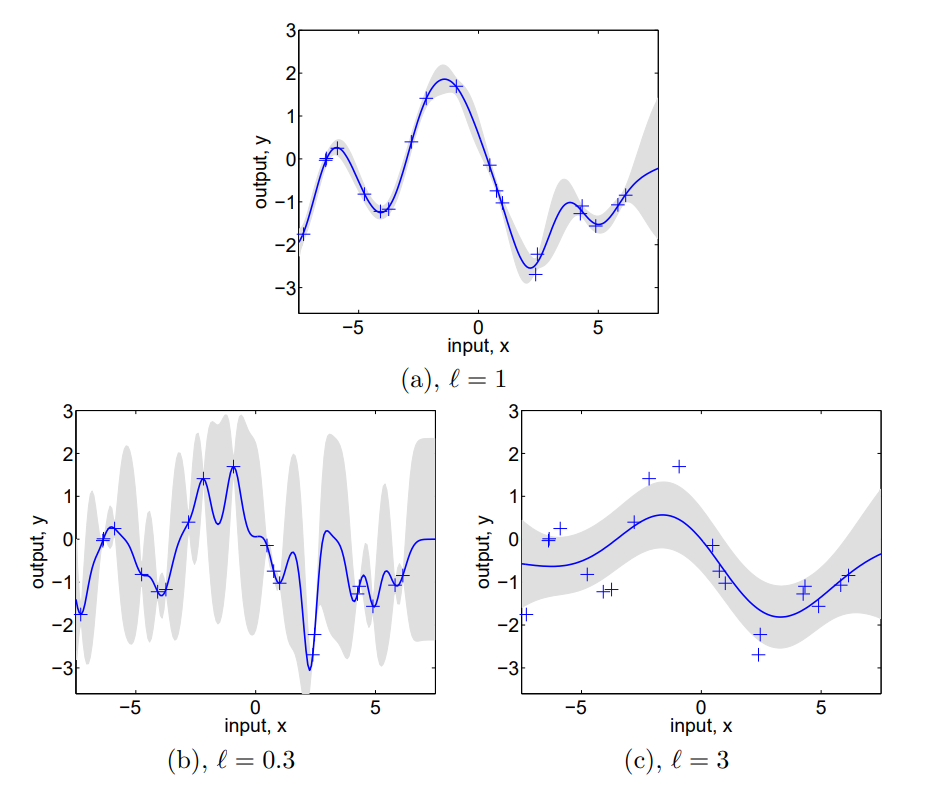
\includegraphics[width=4in]{img/05_4/lengthscale.png}
	\caption[Lengthscale influence on samples]
	{Comparison of hyperparameters for the squared exponential kernel function. A large lengthscale exhibits properties where the function does not react to changes quickly, while a small lengthscale gives the opportunity to react to changes almost immediately. While small lengthscales usually lead to better fits, the prediction power often decreases since more information from noise is incorporated into the covariance matrix. The data is generated from a GP with $l_a=0.3$, $l_b=1$, $l_c=3$, $\sigma_f=1$, and $\sigma_n=0.1$ \cite{Rasmussen_06}. The panel a has lengthscale $l_a$, panel b has lengthscale $l_b$, and panel c $l_c$.}
\end{figure}
The variances, often denoted by $\sigma_n$ for the noise variance, and $\sigma_f$ for the kernel function variance, influence the confidence interval in which we assume the functions to lie. $\sigma_n$ stems from the noise we attribute to the special systemic noise of the problem at hand, while $\sigma_f$ stems from just observing data that is noisy. A large noise variance and kernel variance will exhibit the kernel matrix incorporating a larger error tolerance. This can be seen in the enlargening of the confidence intervals on the draws of functions from the same process. Higher Variances lead to more flexible fitting, while lower variances will be more rigid. On the other hand, if variances are too high or too low, essential information about the structure of the problem can get lost.